
\documentclass[ucs]{beamer}

\usetheme{GSyC}
%\usebackgroundtemplate{\includegraphics[width=\paperwidth]{gsyc-bg.png}}


\usepackage[spanish]{babel}
\usepackage[utf8x]{inputenc}
\usepackage{graphicx}
\usepackage{amssymb} % Simbolos matematicos
\usepackage{enumerate}


% Metadatos del PDF, por defecto en blanco, pdftitle no parece funcionar
   \hypersetup{%
     pdftitle={Virtualización II},%
     %pdfsubject={Diseño y Administración de Sistemas y Redes},%
     pdfauthor={GSyC},%
     pdfkeywords={},%
   }
%


% Para colocar un logo en la esquina inferior de todas las transpas
%   \pgfdeclareimage[height=0.5cm]{gsyc-logo}{gsyc}
%   \logo{\pgfuseimage{gsyc-logo}}


% Para colocar antes de cada sección una página de recuerdo de índice
%\AtBeginSection[]{
%  \begin{frame}<beamer>{Contenidos}
%    \tableofcontents[currentframetitle]
%  \end{frame}
%}


%\newboolean{detallado}
%\setboolean{detallado}{false}
%\newcommand{\opcional}[1]{\ifthenelse{\boolean{detallado}}{#1}{}}


\definecolor{darkred}{rgb}  {1.0, 0.0, 0.0}
\definecolor{darkgreen}{rgb}{0.0, 0.4, 0.0}
\definecolor{darkblue}{rgb} {0.0, 0.0, 0.8}

% for resalted text
\newcommand{\res}[1]{\textcolor{darkred}{#1}}
% for different text
\newcommand{\dif}{\textsl}
% for reserved words
\newcommand{\rw}[1]{\textrm{\textbf{#1}}}
% for commands
\newcommand{\com}[1]{\textrm{\textbf{#1}}}






\begin{document}

% Entre corchetes como argumento opcional un título o autor abreviado
% para los pies de transpa
\title[Virtualización II]{Virtualización II}
%\subtitle{Diseño y Administración de Sistemas y Redes}
\author[GSyC]{Escuela Técnica Superior de Ingeniería de Telecomunicación\\
Universidad Rey Juan Carlos}
\institute{gsyc-profes (arroba) gsyc.urjc.es}
\date[2017]{Noviembre de 2017}



%% TÍTULO
\begin{frame}
  \titlepage
  % Oportunidad para poner otro logo si se usó la opción nologo
  % \includegraphics[width=2cm]{logoesp}  
\end{frame}



%% LICENCIA DE REDISTRIBUCIÓN DE LAS TRANSPAS
%% Nota: la opción b al frame le dice que justifique el texto
%% abajo (por defecto c: centrado)
\begin{frame}[b]
\begin{flushright}
{\tiny
\copyright \insertshortdate~\insertshortauthor \\
  Algunos derechos reservados. \\
  Este trabajo se distribuye bajo la licencia \\
  Creative Commons Attribution Share-Alike 4.0\\
}
\end{flushright}  
\end{frame}



%% ÍNDICE
\begin{frame}
  \frametitle{Contenidos}
  \tableofcontents
\end{frame}






%%---------------------------------------------------------------
\section{Estructura de los laboratorios del GSyC}
%%---------------------------------------------------------------
\begin{frame}[fragile]
\frametitle{Estructura de los laboratorios del GSyC}
\begin{itemize}
\item
Para las prácticas de esta asignatura, tendrás una cuenta en los laboratorios Linux del Departamento GSyC
\item
La misma cuenta la usarás en las prácticas de muchas asignaturas del Departamento, durante toda la carrera/todo el máster
\end{itemize}


  \begin{footnotesize}
  \begin{verbatim}
Campus de Fuenlabrada
Servidor: bilo
Estaciones virtuales: alpha, beta, gamma, delta
Estaciones: alphaNN, betaNN, gammaNN, deltaNN, zetaNN, epsilon NN
  \end{verbatim}
  \end{footnotesize}

Para conocer la dirección IP de la máquina en la que estás
trabajando puedes usar \verb|hostname -i|
\end{frame}

%%---------------------------------------------------------------
\begin{frame}[fragile]
\begin{itemize}
\item
Las direcciones IP de cada máquina pueden consultarse en el fichero \verb|/etc/hosts| de cualquier equipo

\begin{itemize}
\item
Este fichero equivale a 

\begin{footnotesize}
\verb|%SystemRoot%\system32\drivers\etc\hosts|  (MS Windows)

\verb|/private/etc/hosts|  (Mac OS)

\end{footnotesize}
\end{itemize}

\item
La misma cuenta permite entrar en todas las máquinas
\item
Cada usuario verá el mismo \emph{home} en todas las máquinas de Fuenlabrada
\item
Cada usuario verá el mismo \emph{home} en todas las máquinas de Móstoles, distinto
al de Fuenlabrada
\item
Los servidores están dimensionados para mover ficheros del orden de KBytes o MBytes, no GBytes
\item
Los ficheros de los directorios  \verb|/tmp/| y \verb|/var/tmp| son locales
a cada ordenador
\item
Como en todo linux, 
\begin{itemize}
\item
El directorio \verb|/tmp| se borra cada vez que se reinicia el ordenador
\item
El directorio \verb|/var/tmp| se borra cada vez que al administador le parece oportuno, sin que debamos esperar aviso previo
\end{itemize}


\end{itemize}

\end{frame}



%%%---------------------------------------------------------------
%\section{Configuración de VMware}
%%%---------------------------------------------------------------
%
%
%%%---------------------------------------------------------------
%\begin{frame}[fragile]
%\frametitle{Clonación de una máquina virtual con vmplayer de VMware}
%Basta copiar dos ficheros (preferentemente dentro del mismo directorio)
%\begin{itemize}
%\item
%\verb|mi_maquina.vmx|
%
%Fichero de configuración. Texto editable. Permite cambiar configuración de red, dirección MAC,
%memoria disponible, etc
%
%Cambiando el nombre de este fichero cambiamos el nombre (externo) de la máquina virtual. Pero no debemos cambiar el nombre del resto de ficheros
%\item
%\verb|mi_maquina.vmdk|
%
%Imagen del disco
%\end{itemize}
%
%Una vez encendida la máquina, se crean diversos ficheros adicionales con el estado
%
%\end{frame}
%
%%---------------------------------------------------------------

%%%---------------------------------------------------------------
%\begin{frame}[fragile]
%
%\res{Modos de red}
%\begin{itemize}
%\item
%Bridge. El guest está en misma red que host.  Interfaz  VMnet0
%\item
%Nat.  Interfaz VMnet8
%\item
%host only. Interfaz VMnet1
%\end{itemize}
%%
%\res{Puesta en marcha}
%\begin{itemize}
%\item
%Para poner en marcha la máquina
%
%\verb|vmplayer mi_maquina.vmx &|
%\item
%Para que el foco (ratón y teclado) pase a la máquina virtual, pulsamos \verb|ctrl g|
%\item
%Para que el foco vuelva al host, pulsamos \verb|ctrl alt|
%
%\end{itemize}
%
%
%\end{frame}


%%---------------------------------------------------------------
\section{Configuración de VirtualBox}
%%---------------------------------------------------------------

%%---------------------------------------------------------------

\subsection{Imágenes de máquinas virtuales}
%%---------------------------------------------------------------
\begin{frame}[fragile]
\frametitle{Imágenes de máquinas virtuales}
\begin{itemize}
\item
Una de las ventajas de las máquinas virtuales es que pueden
clonarse (copiarse) de un 
\emph{host}
a otro. Para ello basta copiar un fichero o ficheros: la \emph{imagen de la máquina}

\item
VirtualBox llama a estas imágenes \emph{servicio virtualizado}.
En VirtualBox 4, es un fichero \verb|.ova| 
\footnote{En VirtualBox 3 eran 3 ficheros: .ovf .vmdk .mf}
\end{itemize}
%\begin{enumerate}
%\item
%\verb|.ovf    | Fichero principal de configuración
%
%\item
%\verb|.vmdk   | Imagen del disco duro virtual
%\item
%\verb|.mf     | Hash SHA1 de los ficheros anteriores (opcional)
%\end{enumerate}
%\end{itemize}

\end{frame}


%%---------------------------------------------------------------
\begin{frame}[fragile]
\frametitle{}
Para clonar una máquina virtual de un
\emph{host}
a otro
\begin{itemize}
\item
En el 
\emph{host}
origen, exportamos la imagen
%Exportamos el \emph{guest}, 
indicando dónde queremos guardar el .ova 


\item
Llevamos este ficheros al 
\emph{host} 
destino 

\item
Importaremos el .ova, esto generará automáticamente una nueva copia 
del disco duro virtual, en el directorio especificado en

\begin{scriptsize}
\begin{verbatim}
Archivo|Preferencias|General|
Carpeta predeterminada de máquinas
\end{verbatim}
\end{scriptsize}
\item
Podemos borrar el .ova, pero normalmente será preferible
conservarlo por si queremos en el futuro otrá máquina \emph{como nueva}


\end{itemize}

Observa que entonces tenemos 3 copias del disco duro virtual
\begin{enumerate}
\item
La del 
\emph{host}
origen, en formato \verb|.vmdk|
\item
La \emph{que viaja}, incluida dentro del fichero \verb|.ova|
\item
La del
\emph{host}
destino, en formato \verb|.vmdk|
\end{enumerate}


\end{frame}


%%---------------------------------------------------------------
%\begin{frame}[fragile]
%\frametitle{Instalación de una m.v. partiendo desde cero}
%\begin{itemize}
%\item
%Instalamos VirtualBox
%\item
%Lanzamos el asistente para crear una máquina virtual

%\verb|koji@mazinger:~$ virtualbox &|
%\item
%Por omisión, la configuración de la máquina virtual se guarda en 
%
%\verb|~/.VirtualBox/Machines/|
%\item
%Usamos un cdrom o una imagen \verb|.iso| con el disco de instalación del guest
%\item
%Creamos un disco duro virtual, por omisión el asistente lo deja en
%
%\verb|~/.VirtualBox/HardDisks/|
%
%\end{itemize}

%\end{frame}



%%---------------------------------------------------------------
%\begin{frame}[fragile]
%\frametitle{Instalación de una m.v. partiendo de un disco virtual}
%\begin{itemize}
%\item
%En esta asignatura, para ahorrar tiempo partiremos de un disco duro virtual
%de una máquina ya instalada
%
%p.e. \verb|/var/tmp/jeos/jeos.8.04.vdi|
%\item
%La ubicación por defecto del disco duro virtual no es apropiada para
%el laboratorio, el servidor de NFS tendría muchos problemas para mover
%tantos ficheros tan grandes  (en tu casa no tendrías este problema)
%
%Así que guardaremos el disco duro virtual en un fichero local de cada puesto
%del laboratorio
%
%p.e. \verb|/var/tmp/TULOGIN/jeos.8.04.vdi|
%
%\end{itemize}
%
%\res{No confundas ambos ficheros}. Al primero solo tendrás acceso de lectura, para
%que puedas hacer una copia, el segundo, con la que trabajarás
%
%
%\end{frame}



%%---------------------------------------------------------------
\begin{frame}[fragile]
\frametitle{Ejemplo típico de uso de máquinas virtuales}
\begin{itemize}
\item
Un profesor instala una máquina virtual partiendo de cero 

Crea una máquina, especifica su tamaño de disco, de memoria, etc

\item
El profesor exporta la máquina virtual como fichero .ova (que dentro lleva un 
 .vmdk )
y la deja en algún lugar, como p.e. el directorio \verb|/var/lib/vms|
de las máquinas de sus alumnos

\item
Cada alumno instala la máquina virtual en su VirtualBox partiendo de la imagen creada
por el profesor

%con lo que 
%automáticamente se creará una copia de la máquina virtual en el
%\emph{host} del alumno. 

\item
Ahora el alumno podría exportar de nuevo la máquina virtual y llevársela
en un \emph{pendrive} al pc de su casa
\end{itemize}

Algo muy parecido podría hacerlo un administrador con los equipos de
sus usuarios, o un administrador que quiera conservar un servidor
recién instalado para recuperarlo rápidamente si hay problemas

\end{frame}
%%---------------------------------------------------------------
\begin{frame}[fragile]
\frametitle{Instalación de una m.v. partiendo de cero}
Si ya contamos con una imagen de la m.v, podemos omitir estos pasos. Pero en otro caso:
\begin{enumerate}
\item[1]
Lanzamos \verb|VirtualBox| desde la shell

\item[2]
Pulsamos el botón \emph{nueva}, que ejecuta el 
asistente para crear una nueva máquina virtual

\item[3]
Indicamos el nombre de la m.v. (p.e. \verb|pc01|, \verb|ro01|, \verb|auditor01|) 

Sistema operativo Linux, Versión Ubuntu

\item[4]
El tamaño de memoria base dependerá de lo que tenga el \emph{host} y necesite en \emph{guest}. 
Como referencia:

\begin{itemize}
\item
OpenWrt: 32 Mb
\item
Ubuntu Server: 192 Mb
\item
Ubuntu con gráficos, BackTrack con gráficos: 512 Mb

\end{itemize}
\end{enumerate}


\end{frame}
%%----------------------------------------------
\begin{frame}[fragile]

\begin{enumerate}
\item[5]
Activamos \emph{Crear disco virtual} y seguimos el asistente

El tamaño del disco dependerá de lo que tenga el \emph{host} y necesite en \emph{guest}.
Como referencia:

\begin{itemize}
\item
OpenWrt: 64 Mb
\item
Ubuntu, Backtrack: 8Gb
\end{itemize}


\item[6]
En la ventana \emph{resumen} revisamos todo y pulsamos
\emph{Terminar}

%\item
%Activamos \emph{Usar un disco duro existente}
%pulsamos el icono que representa un directorio.
%Esto abre la ventana \emph{Manejador de Medios Virtuales}
%donde pulsamos
%\emph|Agregar| 
%e indicamos la ubicación del disco duro virtual 
%(extensión .vdi)

\end{enumerate}


\end{frame}
%%----------------------------------------------
\begin{frame}[fragile]
Una vez que hemos especificado los componentes
de la máquina, habrá que instalar el sistema operativo, que
normalmente tendremos en un cdrom/dvd o en una imagen iso de
un cdrom/dvd
\begin{itemize}
\item
En el apartado de configuración
de la máquina virtual, en

\begin{scriptsize}
\verb@Almacenamiento | controlador IDE @

\verb@(pulsamos en el icono que representa un CD con el signo +)@

\verb@(pulsamos en el CD recién creado, llamado "vacio")@

\verb@(Vamos a "dispositivo cd/dvd@")
\end{scriptsize}

Aquí indicamos si usaremos el lector físico del \emph{host} (anfitrión)
o una imagen iso del cdrom/dvd

\end{itemize}

\end{frame}






%%---------------------------------------------------------------
\begin{frame}[fragile]
\frametitle{Instalación de una m.v. partiendo de una imagen}
Desde VirtualBox

\begin{itemize}
\item
Comprobamos en 
\begin{scriptsize}
\begin{verbatim}
Archivo|Preferencias|General|
Carpeta predeterminada de máquinas
\end{verbatim}
\end{scriptsize}
que el disco duro virtual quedará copiado en el lugar adecuado.

\begin{itemize}
\item
En casa, el lugar por omisión es válido:

\verb|~/VirtualBox VMs|
\item
En el laboratorio, es imprescindible que sea \verb|/var/tmp/tulogin|
\end{itemize}


\item

  \begin{footnotesize}
  \begin{verbatim}
Archivo|Importar servicio virtualizado|Seleccionar
  \end{verbatim}
  \end{footnotesize}
(Elegimos el fichero .ova)
\item
En la ventana \emph{Configuración de importación de servicios virtualizados}
podemos cambiar algunos parámetros del \emph{guest} (nombre, memoria, disco....)
\end{itemize}

\end{frame}

%----------------------------------------
\begin{frame}[fragile]
\frametitle{}
\begin{center}
\begin{figure}
\centerline{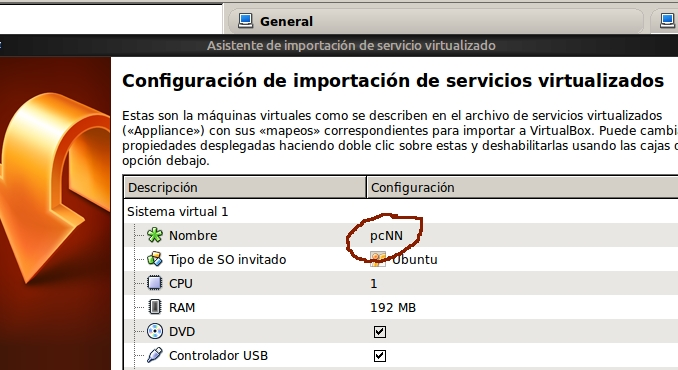
\includegraphics[width=8.5cm]{figs/vbox01}}
\end{figure}
\end{center}

\begin{itemize}
\item
Si dos máquinas van a compartir segmento de red, es necesario cambiar su dirección MAC
\item
Si la imagen original se llama p.e. \verb|pcNN|, haciendo clic
sobre este nombre en la pantalla de configuración de importación,
podemos cambiarlo. P.e. para llamarla \verb|pc01|

\end{itemize}


\end{frame}

%%----------------------------------------------
\begin{frame}[fragile]

Este es el nombre de la máquina visto desde VirtualBox.

Para cambiar el nombre visto desde dentro de la propia máquina,
hay que 

\begin{itemize}
\item
O bien 
editar \verb|/etc/hostname| 

Esto es persistente pero tiene efecto en el próximo reinicio
\item
O bien ejecutar la orden

\verb|hostname <NUEVO_NOMBRE>|

Esto es inmediato pero no es persistente

\end{itemize}
\end{frame}



%%----------------------------------------------
\begin{frame}[fragile]

\frametitle{Fragmentación de ficheros }
Si necesitas trocear una imagen de gran tamaño en ficheros que quepan en un 
\emph{pendrive} o cdrom

\begin{itemize}
\item
Empaquetar y comprimir un directorio:\\ \verb|tar -cvzf mi_imagen.tgz mi_directorio|
\item
Mostrar contenido:\\ \verb|tar -tzf mi_imagen.tgz|

\item
Trocear:\\
\verb|#     tamaño    fichero        prefijo|
\verb|split -b 500MB  mi_imagen.tgz  mi_imagen.tgz.|
\begin{footnotesize}
(Observa que el segundo parámetro es igual al primero, pero
añadiendo un punto)
\end{footnotesize}


\item
Habremos generado
  \begin{footnotesize}
  \begin{verbatim}
mi_imagen.tgz.aa  mi_imagen.tgz.ab  mi_imagen.tgz.ac
  \end{verbatim}
  \end{footnotesize}
\end{itemize}
\end{frame}

%%----------------------------------------------
\begin{frame}[fragile]
En la máquina destino (no importa si en el \emph{host} el S.O. es distinto)
\begin{itemize}
\item
Unir los fragmentos
\verb|cat mi_imagen.tgz.* > mi_imagen.tgz|

(En MS Windows para este paso podemos emplear HjSplit, Free File Splitter o cualquier otro programa similar)
\item
Descomprimir y desempaquetar:\\ \verb|tar -xvzf mi_imagen.tgz |

(En MS Windows podemos usar 7-Zip  o similares)
\end{itemize}

\end{frame}


%%---------------------------------------------------------------
%\begin{frame}[fragile]
%\frametitle{Uso de VirtualBox en los laboratorios del GSyC}
%En el sistema de ficheros del \emph{host}, una máquina virtual consta de
%\begin{itemize}
%\item
%Un directorio con unos cuantos ficheros de configuración
%
%Almacenado por omisión en \verb|~/.VirtualBox/Machines|
%\item
%Un fichero por cada disco duro que tenga el \emph{guest}
%
%Almacenado por omisión en \verb|~/.VirtualBox/HardDisks|
%Puede ser de dos tipos
%\begin{itemize}
%\item
%Almacenamiento de expansión dinámica
%
%Fichero que ocupa tanto como ocupen los datos escritos dentro del disco virtual. Va creciendo, hasta un máximo
%\item
%Almacenamiento de tamaño fijo

%Fichero que ocupa tanto como el tamaño máximo del disco virtual
%\end{itemize}
%\end{itemize}
%
%\end{frame}

%%---------------------------------------------------------------

\subsection{Interfaces de red en VirtualBox}
%%---------------------------------------------------------------

\begin{frame}[fragile]
\frametitle{Interfaces de red de VirtualBox}
\begin{center}
\begin{figure}
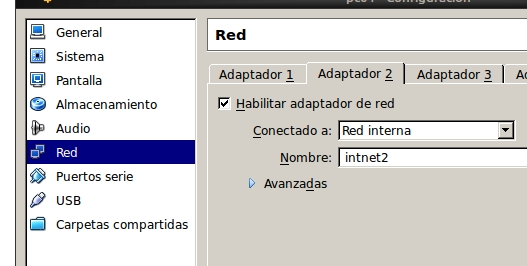
\includegraphics[width=8cm]{figs/vbox02}
\end{figure}
\end{center}
\begin{itemize}
\item
Cada máquina virtual puede tener hasta 4 interfaces \emph{aka} adaptadores de red

\emph{adaptador 1} será eth0, \emph{adaptador 2} será eth1, etc
\item
Cada interfaz puede conectarse a 5 tipos de segmento de red: No conectado,
NAT, Adaptador puente, Red interna, Solo anfitrión
\end{itemize}
\end{frame}

%%---------------------------------------------------------------
\begin{frame}[fragile]
\begin{itemize}
\item
\res{Not attached / No conectado}

Emula una tarjeta con el cable de red desconectado
\item
\res{Network Address Translation (NAT)}

Configuración por defecto. El \emph{guest} tiene acceso al exterior (típicamente internet) a través 
de NAT. El 
\emph{host}
no tiene acceso al
\emph{guest}

Podemos usar varios \emph{guest}, pero cada uno tiene su propio
NAT y está aislado en su propio segmento de red

\item
\res{Bridged networking / Adaptador puente}

Interfaz en el \emph{guest} conectado virtualmente al mismo \emph{hub} (real) que el \emph{host}

El \emph{guest} está en el segmento de red \emph{normal} del \emph{host}

\item
\res{Internal networking / Red interna}

Red entre diferentes \emph{guests} en un mismo \emph{host}

Sin acceso al \emph{host} ni al exterior
%http://www.virtualbox.org/manual/ch06.html
% la red la ven solo las máquinas virtual box, no la ve el host
\item
\res{Host-only networking / Sólo anfitrión}
% red solo entre guest y host. el guest no puede salir

Red entre el \emph{guest} y el \emph{host}, sin acceso al exterior

Permite tener varios \emph{guests} en el mismo segmento
de red
\end{itemize}


\end{frame}
%%---------------------------------------------------------------

\begin{frame}[fragile]
\frametitle{}
Supongamos que deseamos configurar dos 
\emph{guest}
de esta forma:
\begin{center}
\begin{figure}
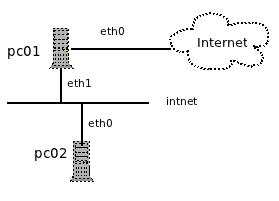
\includegraphics[width=5cm]{figs/scen00}
\end{figure}
\end{center}

\begin{itemize}
\item
En pc01, el interfaz eth0 estaría conectado a NAT

Dentro de la máquina virtual, lo configuraríamos para obtener sus parámetros por DHCP
\item
En pc01, el interfaz eth1 lo conectaríamos a una red interna. El nombre
por omisión de este segmento de red es \emph{intnet} (atención, significa
\emph{internal net}, no \emph{internet})

Podemos ponerle el nombre que queramos al segmento
\end{itemize}
\end{frame}


%%---------------------------------------------------------------
\begin{frame}[fragile]
\frametitle{}
\begin{itemize}
\item
Dentro de la máquina virtual pc01, configuraríamos estáticamente
los parámetros de eth1
\item
En pc02, conectaríamos eth0 a una red interna, con el mismo
nombre que la red interna de eth1 en pc01 (en este ejemplo, \emph{intnet})
\item
Dentro de pc02, configuraríamos estáticamente los parámetros
de eth0
\end{itemize}

\end{frame}


%%---------------------------------------------------------------

\subsection{Configuración que seguiremos en prácticas}
%%---------------------------------------------------------------
\begin{frame}[fragile]
\frametitle{Uso de VirtualBox en los laboratorios del GSyC}
Un disco duro virtual será típicamente un fichero de varios GBytes
almacenado en 

%\verb|~/.VirtualBox/HardDisks|
\verb|~/VirtualBox VMs|
\begin{itemize}

\item
En tu PC esto no será un problema

\item
En el laboratorio sí, el rendimiento sería muy pobre. Por tanto
cambiaremos la ubicación por omisión de los discos duros virtuales

\begin{itemize}
\item
En el  \emph{host}

%\verb|mortuno@iota01:~$ mkdir /var/tmp/$USER|
\begin{scriptsize}
\verb|mkdir /var/tmp/tulogin|

(Donde \emph{tulogin} es tu usuario del laboratorio, p.e.  mgarcia, jperez...)
\end{scriptsize}
\item


En VirtualBox:

\begin{scriptsize}
\begin{verbatim}
Archivo|Preferencias|General|
Carpeta predeterminada de máquinas
\end{verbatim}
\end{scriptsize}


Indicamos

\begin{scriptsize}
\verb@/var/tmp/tulogin@
\end{scriptsize}

\begin{scriptsize}

\textcolor{red}{Muy importante}: asegúrate de cambiar
esta preferencia y mantenerla siempre. De lo contrario, cargarás mucho el
servidor, perjudicandote a tí y a tus compañeros
\end{scriptsize}
\end{itemize}
\end{itemize}
\end{frame}


%%---------------------------------------------------------------
\begin{frame}[fragile]
\frametitle{Problema: las imágenes son ficheros grandes}
Con lo visto hasta ahora, ya podríamos hacer las prácticas de la 
asignatura. Pero sería poco práctico. 

Supongamos una práctica
que consista en configurar en red 3 máquinas virtuales
\begin{itemize}
\item
Cada alumno tendría que guardar en su cuenta del laboratorio 3 imágenes (con sus 3 discos duros virtuales completos)

\item
Para trabajar en casa, tendría que llevarse las 3 imágenes con sus 3 discos duros virtuales completos

\item
Para que 70 alumnos entreguen su práctica, el profesor tendría que manejar 210 discos duros virtuales completos
\end{itemize}

Si en la asignatura se hacen 2 o 3 prácticas, seguimos multiplicando...
\end{frame}

%%---------------------------------------------------------------
\begin{frame}[fragile]
\frametitle{Solución: almacenar solo los ficheros importantes}
Administrar un Unix/Linux consiste en editar diversos ficheros de texto

\begin{itemize}
\item
Solamente manejaremos estos ficheros, que estarán guardados en la cuenta
de bilo y respaldados en la nube de Dropbox
\item
Las máquinas virtuales serán \emph{de usar y tirar}, tomarán la configuración
de estos ficheros
\item
Dentro de las máquinas virtuales, los ficheros de configuración
serán enlaces simbólicos a ficheros en un directorio, que a su vez
estará montado por red desde un directorio en el laboratorio
\end{itemize}

\end{frame}

%%---------------------------------------------------------------
\begin{frame}[fragile]
\frametitle{Ejemplo:}

Para configurar los interfaces de red de una máquina, hay que
editar \verb|/etc/network/interfaces|
\begin{itemize}
\item
Dentro de la máquina virtual \verb|pc01|, este fichero será un
enlace simbólico que apuntará a \verb|/media/nube/interfaces|
\item
El directorio \verb|/media/nube| de \verb|pc01|, estará montado
desde el directorio \verb|~/Dropbox/pc01| del laboratorio
\item
Por tanto, \verb|/etc/network/interfaces| en la máquina
virtual pc01 y \verb|~/Dropbox/pc01/interfaces| en el laboratorio
serán el mismo fichero, podrá editarse indistintamente cualquiera de los dos
\end{itemize}

\end{frame}


%%---------------------------------------------------------------
%\begin{frame}[fragile]
%Una vez creada una máquina, si te sientas en un puesto distinto del laboratorio 
%\begin{itemize}
%\item
%Es necesario
%que vuelvas a copiar a mano el disco duro virtual (recuerda que \verb|/var/tmp| es 
%local en cada máquina)
%\item
%La máquina virtual seguirá siendo visible, puesto que está definida en
%tu \emph{home}, en el fichero
%
%\verb|~/.VirtualBox|
%
%\end{itemize}
%
%
%Recuerda que 
%
%\begin{itemize}
%\item
%El administrador puede borrar tu máquina virtual en cualquier
%momento, no guardes dentro nada de valor
%\item
%Para usar tus \emph{guest} en los distintos \emph{hosts} del laboratorio,
%no necesitas importar y exportar máquinas completas. La máquina virtual
%está en tu \emph{home}, lo único que tienes que copiar a mano es el disco duro
%virtual (ubicado en \verb|/var/tmp/TULOGIN|)
%\end{itemize}
%\end{frame}



%%----------------------------------------------
\begin{frame}[fragile]

Para montar el directorio remoto, aquí emplearemos sshfs

Ventaja principal:
\begin{itemize}
\item
Basta con tener acceso por ssh a la máquina remota para poder montar un directorio
\end{itemize}


Pero esta idea de tener los ficheros importantes por
separado y luego colocarlos automáticamente en su sitio puede aplicarse de muchas otras formas
\begin{itemize}
\item
Tanto en máquinas físicas como virtuales
\item
En un entorno docente, doméstico, de oficina, granja de servidores...
\item
Mediante nfs, o scp, o rsync, o unison, o smb/cifs, o vboxsf...
\item
Con la oportuna atención a la seguridad si se trata de un sistema en producción
\end{itemize}

\end{frame}



%%----------------------------------------------
\begin{frame}[fragile]
\frametitle{Montar un directorio con sshfs}
Punto de montaje: directorio local donde veremos el directorio remoto

\begin{itemize}
\item
Montar el \emph{home} remoto:

  \begin{footnotesize}
  \begin{verbatim}
sshfs  usuario@maquina: /punto/de/montaje
  \end{verbatim}
  \end{footnotesize}


\item
Montar un directorio remoto cualquiera


  \begin{footnotesize}
  \begin{verbatim}
sshfs  usuario@maquina:/un/directorio  /punto/de/montaje
  \end{verbatim}
  \end{footnotesize}

(Siempre path absoluto, no soporta \verb|~|)

\item
Desmontar:

  \begin{footnotesize}
  \begin{verbatim}
fusermount -u /punto/de/montaje
  \end{verbatim}
  \end{footnotesize}
\end{itemize}

No siempre es necesario tener privilegios de root (es configurable)

En conexiones lentas puede ser conveniente añadir la opción -C para
que comprima el tráfico

  \begin{footnotesize}
  \begin{verbatim}
sshfs -C usuario@maquina:/path  /punto/de/montaje
  \end{verbatim}
  \end{footnotesize}
\end{frame}

%%---------------------------------------------------------------
%\begin{frame}[fragile]
%\frametitle{}
%
%Para facilitar el trabajo, las máquinas que usarás ya tendrán los
%enlaces simbólicos preparados.
%Para montar el directorio remoto, basta con edites y luego ejecutes
%(como administrador) el script \verb|~user/monta|
%
%Sus primeras líneas son
%  \begin{scriptsize}
%  \begin{verbatim}
%#!/bin/bash
%#USUARIO=     #Tu login del laboratorio
%#HOST=193.147.49.NN     #Dirección IP o nombre completo de tu host en el labo.
%#HOME_REMOTO=/home/al-05-06/TULOGIN  #PATH absoluto de tu home en el labo.
%#GUEST_NAME=pc01   #Nombre de este guest. P.e. pc01, pc02, etc
%###############################################################
%  \end{verbatim}
%  \end{scriptsize}
%
%Una vez editado, resultará p.e.
%
%  \begin{footnotesize}
%  \begin{verbatim}
%#!/bin/bash
%USUARIO=jperez
%HOST=193.147.49.21    
%HOME_REMOTO=/home/al-05-06/jperez  
%GUEST_NAME=pc01  
%  \end{verbatim}
%  \end{footnotesize}
%(No puede haber espacios ni a la derecha ni a
%la izquierda del igual)
%
%
%
%\end{frame}


%%---------------------------------------------------------------
%\begin{frame}[fragile]
%\frametitle{}
%En nuestro caso, \verb|/media/nube| es el \emph{punto de montaje}
%
%\begin{itemize}
%\item
%Un punto de montaje 
%es un directorio en una máquina. Tiene que existir, suele
%estar vacío, pero podría tener ficheros
%\item
%Cuando \emph{montamos otro sistema de ficheros encima del punto
%de montaje},  el nuevo sistema de ficheros (el directorio
%compartido) pasa a verse en ese punto del árbol del sistema
%de ficheros
%
%El contenido previo del punto de montaje deja
%de estar accesible, pero no se borra
%\item
%Si \emph{desmontamos} el sistema de ficheros, el contenido previo
%del punto de montaje vuelve a estar accesible
%\end{itemize}
%
%\end{frame}


%%---------------------------------------------------------------
%\begin{frame}[fragile]
%\begin{itemize}
%\item
%Para configurar el directorio en el
%\emph{host},
%indicaremos
%la ruta en el 
%\emph{host}
%y el
%\emph{folder name/nombre carpeta}
%
%\item
%Para montar el directorio en el 
%\emph{guest},
%indicaremos el 
%\emph{folder name/nombre carpeta}
%y la ruta
%en el 
%\emph{guest}
%
%\item
%\res{Error frecuente :} Indicar en alguna máquina
%(\emph{host} o \emph{guest} )
%directamente 
%la ruta en el 
%\emph{host} y la ruta 
%en el
%\emph{guest}, sin usar el nombre de carpeta.
%
%\end{itemize}

%\end{frame}


%

%%---------------------------------------------------------------
\subsection{Cambio de host en el laboratorio}
%%---------------------------------------------------------------
\begin{frame}[fragile]
\frametitle{Cambio de host en el laboratorio}
La m.v. está en un directorio local del pc donde trabajas, no en tu cuenta
de pantuflo/bilo

Si te sientas en un puesto del laboratorio distinto al del dia anterior:
\begin{enumerate}
\item
Sal de VirtualBox y borra la máquina vieja
  \begin{footnotesize}
  \begin{verbatim}
rm -rf ~/.VirtualBox
rm -rf /var/tmp/tulogin/*  # si este directorio existe
  \end{verbatim}
  \end{footnotesize}

\item
Vuelve a indicar en 
\begin{scriptsize}
\begin{verbatim}
Archivo|Preferencias|General|
Carpeta predeterminada de máquinas
\end{verbatim}
\end{scriptsize}
que la carpeta predetermina de máquinas tiene que ser \verb|/var/tmp/tulogin|

\item
Vuelve a importar el servicio virtualizado
(O copia \verb|/var/tmp/tulogin| desde el host anterior)





\end{enumerate}

\end{frame}


%%---------------------------------------------------------------
\begin{frame}[fragile]
\frametitle{Observaciones}
\begin{itemize}
\item
Recuerda que el administrador puede borrar tu máquina virtual en cualquier
momento, no guardes dentro nada de valor, todos tus ficheros deben estar
en el directorio compartido



\item
En esta asignatura, cada máquina Ubuntu tendrá por omisión un
usuario de nombre
\verb|user|
y contraseña
\verb|user|
autorizado a ejecutar la orden \verb|sudo|      
\begin{itemize}
\item
Recuerda que en el caso de Ubuntu, se espera que no empleemos el usuario \verb|root|
\end{itemize}

\item
En las máquinas sin gráficos, podemos usar varias consolas pulsando
 \verb|Alt F1|,
\verb|Alt F2|, etc
\item
Si dejamos la máquina virtual desatendida algunos minutos, puede 
saltar el salvapantallas y quedarse en negro. En tal caso, llevamos
el foco a la  máquina virtual (haciendo clic dentro) y pulsamos cualquier tecla
\end{itemize}

\end{frame}


%%---------------------------------------------------------------
\begin{frame}[fragile]
\frametitle{Algunos errores posibles}
Si has empezado a importar una máquina virtual, te has equivocado
en algo y has vuelto a empezar, VirtualBox puede mostrará un error
indicando que ese disco duro ya está registrado y no puede importarse de nuevo

Soluciones
\begin{enumerate}
\item
En
  \begin{footnotesize}
  \begin{verbatim}
Archivo | Administrador de medios virtuales
  \end{verbatim}
  \end{footnotesize}
Elimina esa imagen de la lista de medios conocidos, o elimínala por completo (una ventana
te informará). Fíjate si es la imagen \emph{que viaja} o la del \emph{host destino}

\item
Alternativa más drástica: Cerrar VirtualBox y borrar todo el directorio \verb|~/.VirtualBox|

(esto elimina toda la configuración y todas las máquinas)
\end{enumerate}

\end{frame}

%%----------------------------------------------
\begin{frame}[fragile]

Si intentamos usar dos instancias de un \emph{guest} en 
el mismo \emph{host} nos dará un error indicando que ambos
discos tienen el mismo identificador. En este caso, hay que
clonar el disco

Ejecutamos desde la shell

\verb|VBoxManage clonehd   <filename> <outputfilename>|
\end{frame}


%%---------------------------------------------------------------
\section{Algunos bugs conocidos}
%%---------------------------------------------------------------

%%---------------------------------------------------------------
\begin{frame}[fragile]
\frametitle{Reiniciar VirtualBox}
\begin{itemize}
\item
Para borrarlo todo y volver a empezar, elimina los directorios  \verb|~/.VirtualBox| y \verb|/var/tmp/tulogin|

\begin{scriptsize}
Pero recuerda volver a indicar \verb|/var/tmp/tulogin| en
\begin{verbatim}
Archivo|Preferencias|General|
Carpeta predeterminada de máquinas
\end{verbatim}
\end{scriptsize}
\end{itemize}

\end{frame}

%%---------------------------------------------------------------
\section{Configuración del teclado}
%%---------------------------------------------------------------
\begin{frame}[fragile]
\frametitle{Configuración del teclado}
\begin{itemize}
\item
El teclado habitual en los PCs españoles es el pc105 (O el pc102 si no tiene teclas \emph{menú}, \emph{windows})
\item
El equivalente en los PCs estadounidenses es el pc104 y el pc101, respectivamente
\item
Programadores y usuarios normalmente trabaja con versiones del SO adaptadas a su idioma
\item
Un administrador frecuentemente se encontrará con un SSOO en inglés

\begin{itemize}
\item
Normalmente podrá configurarlo para que admita su propio idioma (si no en menús y documentación, sí en la 
configuración del teclado)
\item
Pero mientras lo configura, tendrá que saber manejarse mínimamente con el teclado desconfigurado
\end{itemize}
\end{itemize}

\end{frame}


%%---------------------------------------------------------------
\begin{frame}[fragile]
\frametitle{}
Si el ordenador tiene X Window (Gráficos), podemos configurarlo con
\begin{itemize}
\item
\verb|setxkbmap us    | Fija el teclado en la disposición pc104
\item
\verb|setxkbmap es    | Fija el teclado en la disposición pc105
\end{itemize}


En Debian/Ubuntu podemos usar

\begin{itemize}
\item
\verb|dpkg-reconfigure console-setup|
\item
O más globalmente 

\verb|sudo dpkg-reconfigure locales|
\end{itemize}

En gnome:

\begin{itemize}
\item
  \begin{verbatim}
Sistema |  Preferencias | Teclado | Distribuciones | 
| Añadir | Español | Subir (hasta colocarlo el primero)
  \end{verbatim}

Necesitarás cambiar esto por ejemplo si entras desde casa
al laboratorio por VNC y lanzas una máquina virtual 
\end{itemize}

En OpenWrt esto no está disponible, la mejor opción es entrar por ssh (lo que exige que la red ya funcione)
\end{frame}





%%---------------------------------------------------------------
\begin{frame}[fragile]
\frametitle{}
Si nuestro teclado es español, pero el sistema operativo espera un teclado norteamericano:

  \begin{footnotesize}
  \begin{verbatim}
Obtener    Pulsar
--------------------------
Esc        Esc
:          Ñ
;          ñ
/          _
!          !
|          shift Ç
'          ,    (apóstofre, coma)
  \end{verbatim}
  \end{footnotesize}


\end{frame}


\end{document}
